\chapter{The System Development}\label{cap:development}

Here will be explained the system developed. Where in Section \ref{section:caseStudyScenario} focuses on the case study, establishing the context in which the project was initially conceived. Section \ref{section:softwareArchitecture}, on the other hand, presents the software architecture designed to achieve the previously set objectives. Additionally, Section \ref{section:dataModel} defines the data model adjusted to the business reality, providing a comprehensive view of the involved processes. In Section \ref{section:leftover}, the traceability system for the wood waste resulting from the furniture manufacturing process is discussed. Finally, Section \ref{section:project} examines the features to track a project. 

\section{Case Study Scenario}\label{section:caseStudyScenario}

This master's thesis focuses on the case study of Mofreitas, a Small and \acrfull{smes} specialized in the production of wooden furniture. The furniture manufacturing involves partially manual and automated processes, employing cutting machinery such as routers, \acrfull{cnc} machines, nesting, and edge banding. One of the challenges faced by the company lies in the traceability of the produced components, encompassing aspects such as individual parts, project stages, leftover materials after fabrication, and tertiary materials consumed throughout the project. Thus, there is complexity both in project traceability and inventory management.

To better understand the problem, prior knowledge of the execution flow of the involved steps is necessary. The production process of Mofreitas carpentry begins with the conception of the furniture solution by the client, which can range from detailed projects to manual sketches or vague ideas. To formalize the project, information is established in collaboration with the client through in-person meetings, email exchanges, or phone calls, and the discussed details are recorded in the OneNote\textsuperscript{\textregistered} software \cite{onenote}.

After this phase, the budgeting process begins with the support of a spreadsheet developed in Microsoft Excel\textsuperscript{\textregistered} \cite{excel2023}. Upon client acceptance of the budget, the technical drawing associated with the project is created using the SolidWorks\textsuperscript{\textregistered} software \cite{solidworks}. During this stage, the client is consulted for possible adjustments and corrections to the project and budget.

After completing the technical drawing, the files generated by the Computer-Aided Design (CAD) software in Parasolid format are imported into the AlphaCAM\textsuperscript{\textregistered} software \cite{alphacam}, which is responsible for generating the necessary files for the nesting machines and programming of the \acrfull{cnc} and milling machines. A more detailed view of the machines on the shop floor and the process can be seen in Figure \ref{fig:shopFloor}. In the working environment of the CAM software, the files are manually organized into internal folders according to the thickness of the wooden boards used in the project. Then, the processing by this program generates the base files for the nesting and CNC machines, which are stored in a shared folder identified with the project reference. 

\begin{figure}[!ht]
     \centering
     \begin{subfigure}[b]{0.32\linewidth}
         \centering
         \includegraphics[width=0.95\textwidth]{images/Development/chap4/machine01.jpg}
         \caption{The photo illustrates the control panel of a machine \acrshort{cnc}.}
         \label{fig:machine01}
     \end{subfigure}
     \hfill
     \begin{subfigure}[b]{0.32\linewidth}
         \centering
         \includegraphics[width=0.95\textwidth]{images/Development/chap4/machine02.jpg}
         \caption{Industrial Wide Belt Sander Machine: specialized in  finishing flat surfaces.}
         \label{fig:machine02}
     \end{subfigure}
      \hfill
     \begin{subfigure}[b]{0.32\linewidth}
         \centering
         \includegraphics[width=0.95\textwidth]{images/Development/chap4/machine03.jpg}
         \caption{Mofreitas operator supervising a \acrshort{cnc} machine.}
         \label{fig:machine03}
     \end{subfigure}
     \caption{The displayed images depict a more detailed view of the processes that take place on the factory floor. In these figures, it is possible to observe the machines that are used on a daily basis.}
     \label{fig:shopFloor}
\end{figure}

Furthermore, these documents are used in the production of records called "cut lists" and "accessory lists". These lists allow for easy reference and provide information about the characteristics and quantities of each component of the project. Illustratively, Figure \ref{fig:cutLsitMyCad} shows an example of one of these cut lists. This file, in \acrfull{csv} format, is automatically generated by an integrated software in the SolidWorks\textsuperscript{\textregistered} environment called MyCADTools\textsuperscript{\textregistered} \cite{mycadtools}. It is then used in the S2M CENTER\textsuperscript{\textregistered} software \cite{s2mcenter} to generate the labels that will be used to identify the various wooden elements cut by the CNC machines. Figure \ref{fig:tagExample} shows an example of such a label.

\begin{figure}[ht!]
    \centering
    \includegraphics[width=.65\linewidth]{images/Development/chap4/ListaDeCorte.png}
    \caption{Excerpt from a cut list generated by MyCADTools software.}
    \label{fig:cutLsitMyCad}
\end{figure}

\begin{figure}[ht!]
    \centering
    \includegraphics[width=.65\linewidth]{images/Development/chap4/tagExample.png} 
    \caption{This is an example of a tag generated by the S2M CENTER\textsuperscript{\textregistered} software. The aforementioned label contains pertinent information about the wood component used in the manufacture of the furniture. Among this information, the specification of the material, dimensions and the identification denomination stand out, which establishes a correlation with the CAD drawings.}
    \label{fig:tagExample}
\end{figure}

It is crucial to highlight that a physical replica of these lists is provided to the production area. This document accompanies all the cut components of a specific project, serving as a guide for the operators. It provides information about which pieces need to be produced, what material is used, which operations are performed, and in what sequence. Additionally, these lists allow for tracking the progress of the production.

Other files that need to be accessed during the production phase are made available through the Google Drive\textsuperscript{\textregistered} cloud storage service \cite{google-drive2023}. This resource is used to obtain essential project files, as illustrated in Figure \ref{fig:dataSharing}. However, these approaches to information management pose significant challenges for effective data management.

\begin{figure}[ht!]
    \centering
    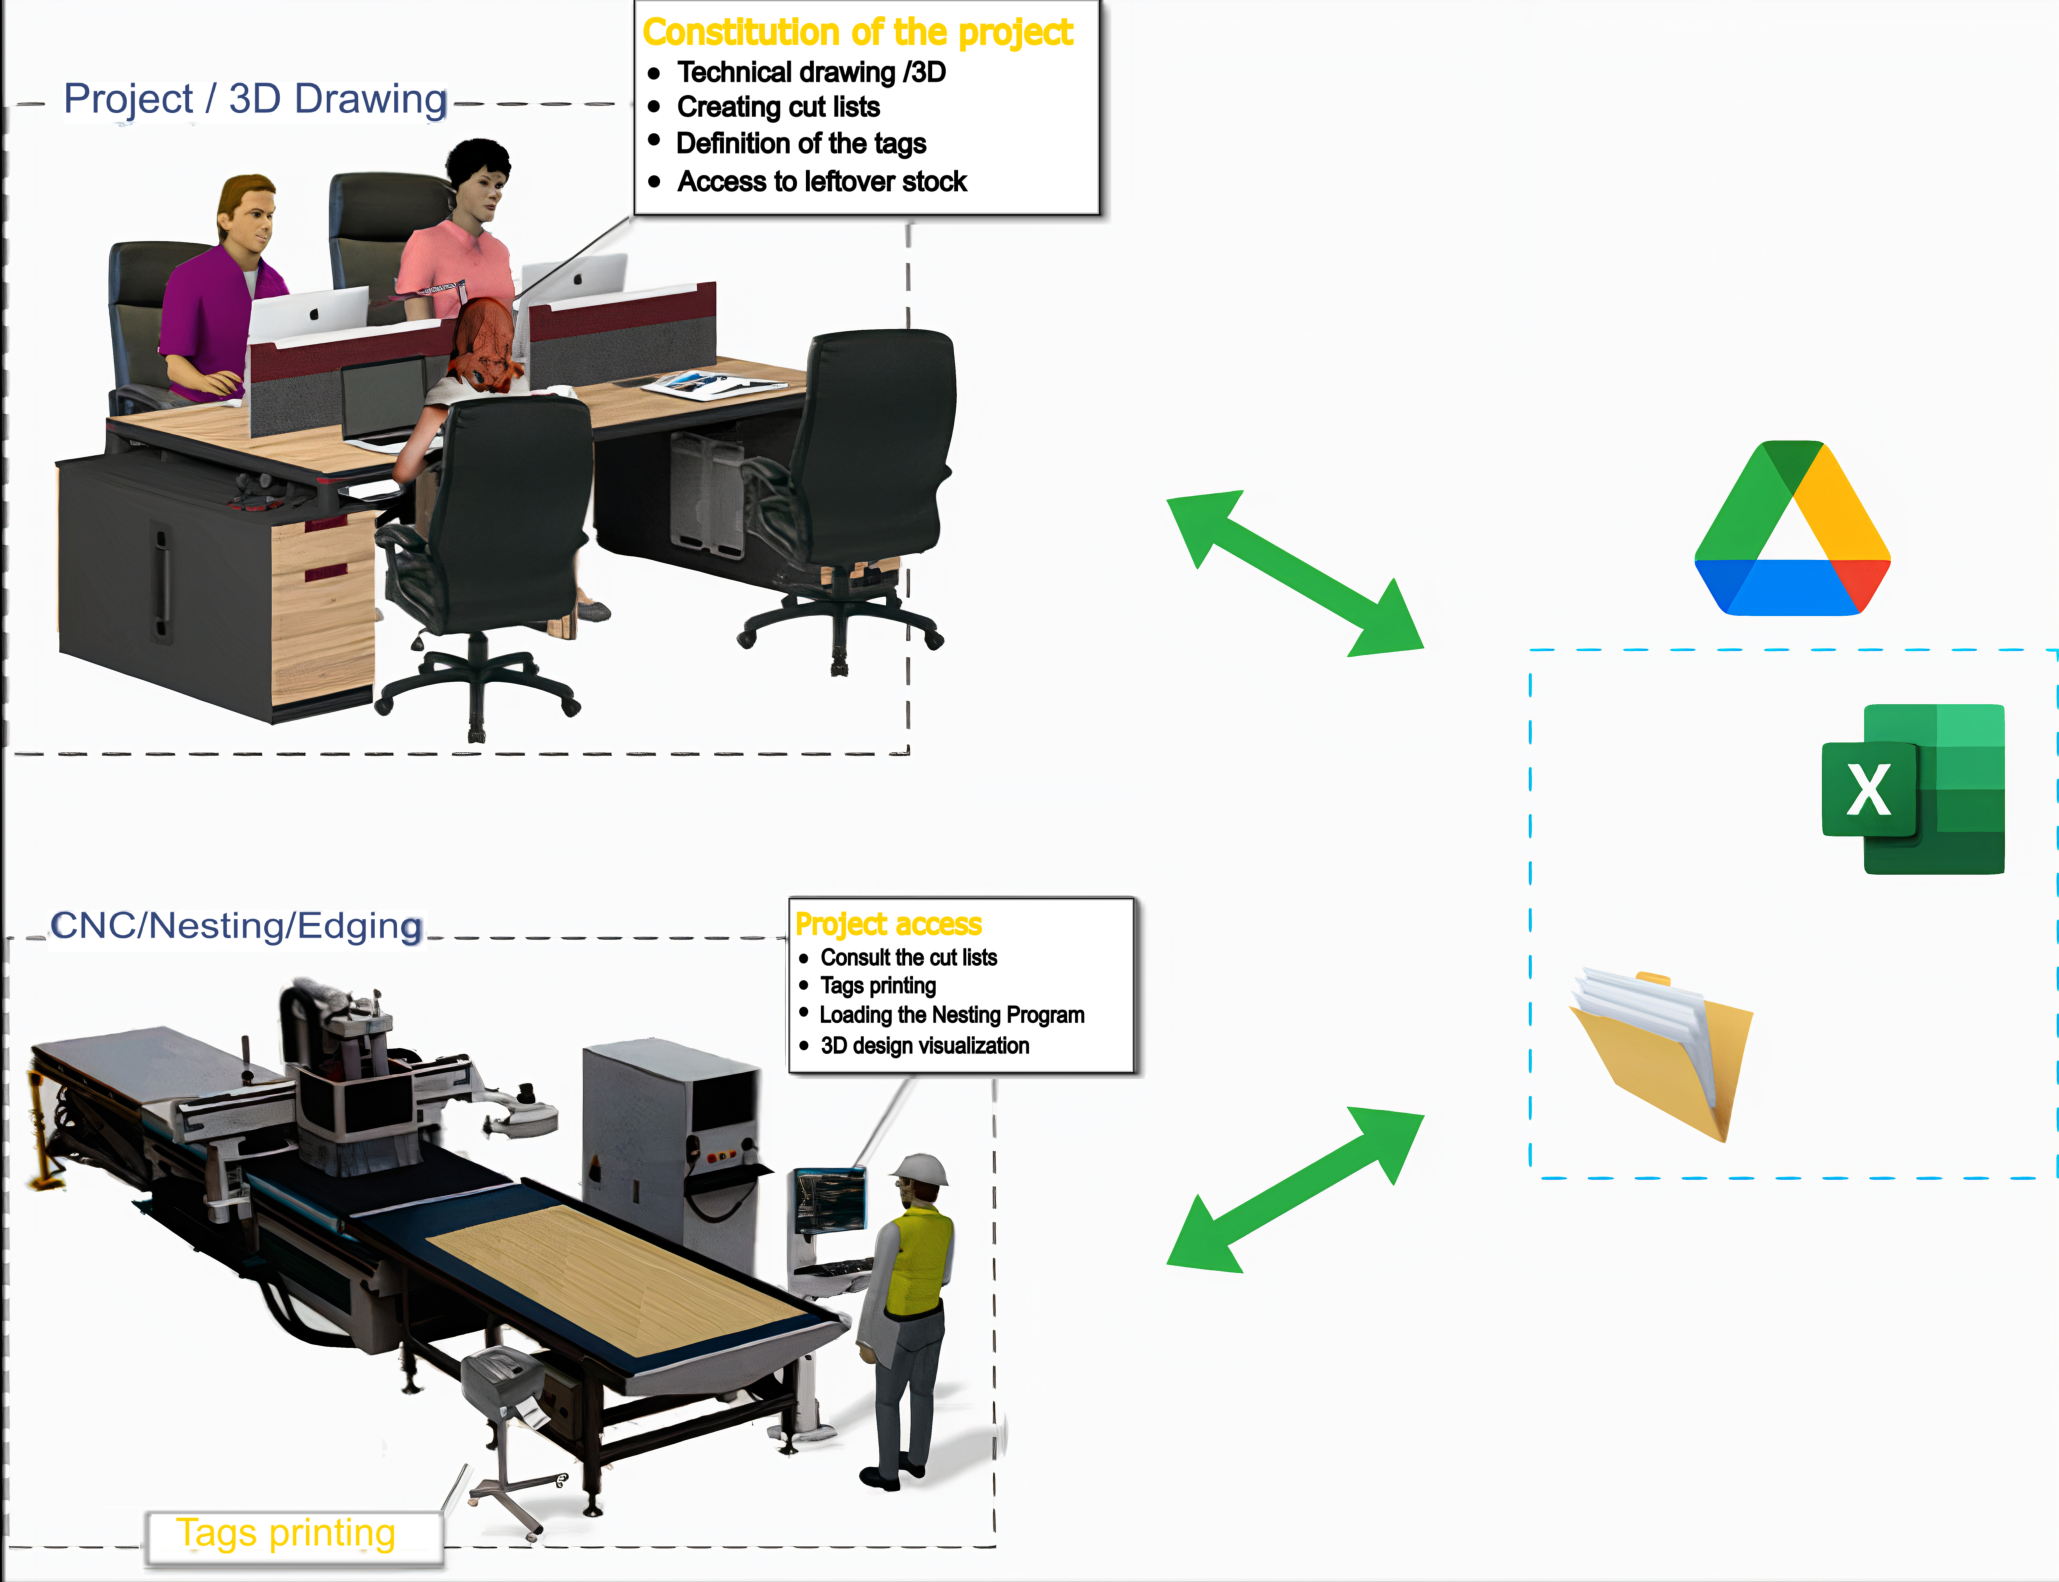
\includegraphics[width=.65\linewidth]{images/Development/chap4/MofreitasCaseIA.pdf}
    \caption{Graphical representation of how mofreitas initially accessed project information in different locations on the factory facility.}
    \label{fig:dataSharing}
\end{figure}

In particular, difficulties arise in situations where synchronization is not executed correctly, network failures occur, or obtaining specific project information becomes complex in an environment filled with data from other projects that are not immediately relevant to the operator. Therefore, handling this information requires a systematic and efficient approach to minimize the possibility of errors and improve the productivity of the production process.

The files produced by AlphaCAM\textsuperscript{\textregistered}, crucial for programming the nesting and CNC machines, are input into the corresponding control software for each machine and operated based on instructions provided by the operators. As mentioned earlier, these files, along with the identification labels that need to be affixed to the pieces after nesting, are accessible on all computers in the production area, located in a cloud-shared folder. Additionally, operators have the ability to consult and view each project in three dimensions by opening the files generated in SolidWorks\textsuperscript{\textregistered} using the eDrawing\textsuperscript{\textregistered} visualization software.


After the cutting and processing of each of the wooden components involved in the project, the assembly process begins, as shown in figure \ref{fig:shopFloor}. The purpose of this phase is to ensure that the furniture production has been carried out in accordance with the project specifications, thus minimizing errors at the final delivery location, which is often a significant distance from the initial manufacturing site.


\begin{figure}[ht!]
    \centering
    \includegraphics[width=.65\linewidth]{images/Development/chap4/mofreitas.png}
    \caption{The image illustrates the preliminary assembly stage at the Mofreitas furniture factory. Operators, among scattered components, check the correct fit of parts and completeness of furniture, essential before the subsequent packaging process. Source: \cite{noauthor_mofreita_2020}.}
    \label{fig:shopFloor}
\end{figure}

This phase often requires the use of various consumables such as screws, anchors, and glue, as well as a range of hardware including hinges, handles, and locks. In terms of inventory management, consumables are purchased from the warehouse by a designated operator in quantities that meet the demand. During this process, the operator is responsible for manually recording the description and quantity of items such as boxes of nails, screws, and other requisitioned items.

As for hardware, the list of materials associated with a specific project is directly processed by the warehouse manager. In this context, all these items are segregated into boxes and associated with the corresponding project through a reference code.

After the assembly, adjustment, and careful inspection of all furniture elements related to the project, the packaging phase begins. In this crucial stage, the components are securely packaged to ensure their integrity during transportation. They are also properly labeled, not only to ensure traceability and facilitate handling during transit but also to assist in correct assembly at the destination site. This labeling is of utmost importance as it contains detailed instructions and the assembly sequence, ensuring that the final assembly is carried out according to the project specifications and preventing the loss of components, which could cause significant logistical disruptions. This packaging process is meticulously planned and executed, aiming not only for the physical protection of the furniture but also for the optimization of space during transportation.

So far, we have covered the various phases of the production process related to the manufacturing of a specific furniture component at Mofreita's carpentry. This journey begins with the project proposal and culminates in the final product, already installed at the customer's location. Among the subprocesses that are essential for the smooth operation and consolidation of this production chain, inventory management stands out.

Primary difficulties are identified in two areas: the first concerns the logistics associated with consumables and hardware, and the second relates to the traceability of wood waste generated from the cutting lists. In terms of the first area, there is a pressing need to digitize the process of requisitioning consumables and hardware to avoid manual recording and to enable real-time integration of this information into the overall management process.

Additionally, the current management of inventory data is carried out using a generic spreadsheet, which hinders the automatic recording of time-related information associated with material inflows and outflows, as well as any price fluctuations. Therefore, updating the inventory management software is a crucial step towards modernizing the production process.

The proposed solution should not only facilitate the storage of inventory-related information but also enable the analysis of this data. This capability allows for the generation of statistics that can support more effective decision-making processes. Data such as the time interval between orders for a specific reference and the average delivery times from a particular supplier are of paramount importance. Given the inherent uniqueness of each project, it is only possible to establish a forecast for the production time. 

Regarding the production chain, the way raw materials are incorporated into the production line is the second issue. Specifically, the fate of the waste generated from each project and how this waste can be automatically reintegrated into the chain is a point of interest. Currently, there is no automatic update of information in the spreadsheet used for inventory control regarding the remaining raw materials from various cutting processes. The leftover wood boards throughout the workweek, which have a usable area, are manually rearranged and reintegrated into the storage area. Their subsequent use is determined by operators through visual inspection for a specific purpose. This operational method is sub-optimal as it results in more waste than if these leftovers were used in nesting processes.

Therefore, the goal is to adopt a strategy for tracking the remaining raw materials so that they can be automatically integrated back into the inventory for more efficient reuse in subsequent manufacturing projects. Specifically, for each waste piece, its dimensions, material type, thickness, and location on the shop floor are intended to be recorded. Additionally, it is crucial to know, if applicable, the wood grain direction. The solution to be developed in the context of Industry 4.0 should allow for the identification of each waste piece on the shop floor and its integration into the inventory list with all the aforementioned characteristics. This information should be utilized to further minimize raw material waste and make the entire process more efficient.


\section{The Software Architecture}\label{section:softwareArchitecture}

As established in the \textcite{ieee} standard, architecture is conceptualized as the fundamental organization of a system, embodied in its components, their relationships with each other and the environment, as well as the principles that guide its design and evolution. In this regard, the development of the software architecture for this project is crucial as it aims to build a system capable of performing a variety of functions simultaneously while adhering to essential criteria: scalability, security, traceability, interaction with a range of devices, and data distribution. This arrangement, by providing a broad spectrum of capabilities, contributes to a robust and versatile system that can adapt and efficiently respond to the variable and complex demands of the manufacturing environment.

\subsection{Scalability}\label{section:softwareArchitecture-scalability}
Scalability, characterized as the ability of a system to adjust its throughput according to emerging needs, expanding or reducing its performance \cite{garland2003large}, has been incorporated into the software architecture to ensure its future expandability and adaptability. These characteristics are particularly necessary in an environment that potentially receives data from sensors, machines, and microservices installed in the manufacturing ecosystem, as well as requests from external networks.

In order to integrate with existing internal services and potentially incorporate new services, specific technologies have been utilized. The \acrfull{fiware}\cite{fiware}, an open platform under the \acrfull{glp}\footnote{The GNU AFFERO GENERAL PUBLIC LICENSE Version 3  also know as General Public License (GPL) is a free software license that guarantees end users the freedom to run, study, share, and modify the software. It was created by the Free Software Foundation (FSF) \cite{tsai2008better}.} license, which provides a set of \glspl{api} that facilitate the development of intelligent applications, has been employed to enable system interoperability and efficient data handling. Additionally, Nginx\textsuperscript{\textregistered} \cite{nginx}, a high-performance web server, has been implemented to manage HTTP requests and load balancing, contributing to the scalability and reliability of the system. The Gunicorn, a Python \acrfull{wsgi} HTTP server\footnote{ WSGI is a specification that defines how web servers and web applications communicate in the Python ecosystem. It establishes a standardized interface that enables web servers like Gunicorn to effectively process requests from Python\textsuperscript{\textregistered} web applications \cite{eby2010pep}.  In other words, WSGI is not a server, a Python module, a framework, an API or any kind of software. It is just an interface specification by which server and application communicate \cite{clodoaldo2015}.}, was also used to serve the web applications of the system, enabling effective communication between the web application and the web server. Each of these technologies plays a vital role in optimizing the system architecture to meet the demands of scalability, adaptability, and integration.

Nginx\textsuperscript{\textregistered} is a widely adopted solution for web server and reverse proxy\footnote{Nginx acts as a simple proxy server, receiving HTTP requests from the client (acting as an HTTP server) and forwarding them to the backend server (acting as an HTTP client). There is therefore no new protocol or software involved. The mechanism is handled by the Nginx Proxy module \cite{fjordvald2018nginx}.}, recognized for its efficient load balancing capabilities in the context of network traffic distribution among multiple servers \cite{Chi2012}. Its Open Source version\footnote{Open-source software is characterized by granting users the right to access and modify the source code of the program, enabling customization according to individual user needs and the dissemination of the modifications made \cite{perens1999open}. This model has gained increasing support, with a growing movement in favor of open-source and a rising number of advocates engaged in this philosophy \cite{lerner2002}. } oferece o  algoritimo Round Robin\footnote{The term "round robin" originated from a historical practice of arranging signatures in a circular form to conceal the order of signing. It is believed to have derived from the French term "ruban rond" or "round ribbon" used in 17th-century France, where government officials signed petitions on ribbons attached to documents in a circular manner \cite[p. 716]{Hendrickson2008}.} for load balancing, which achieves a balanced distribution of incoming requests among the available servers \cite{nginxArticle}. When a client sends a request to the server, it acts as an intermediary, forwarding the request to one of the available backend servers. This approach is reinforced by maintaining persistent connections between the Nginx\textsuperscript{\textregistered} server and each backend server, allowing subsequent requests to be forwarded to the next server, taking into account its availability. Consequently, this strategy results in improved response times and a significant reduction in downtime \cite{Chi2012}.

In addition, load balancing provides redundancy and high availability, allowing the addition or removal of backend servers without interrupting ongoing services. The configuration exemplified in code \ref{code:nginx} demonstrates how the Nginx\textsuperscript{\textregistered} server can be easily set up to implement load balancing effectively \cite{nginxArticle}. For a clear visual understanding of this technology, figure \ref{fig:loadBalancing} offers a graphical representation that makes load balancing operation accessible and comprehensible.

\begin{lstlisting}[style=nginx, label={code:nginx}, xleftmargin=2.75em, language=nginx, caption={This configuration enables load balancing for the 'backend' service using Nginx. This allows to distribute incoming network traffic across multiple servers to improve performance, scalability, and reliability. The service is distributed in two other identical services running in parallel, ww40 and ww41.}, captionpos=b]
worker_processes auto;
http {
    upstream backend {
        server ww40;
        server ww41;
    }
    server {
        listen 80;
        location / {
            proxy_pass http://backend;
            # ... rest of the code.
        }
    }
}
\end{lstlisting}

\begin{figure}[ht!]
    \centering
    \includegraphics[width=.65\linewidth]{images/Development/chap4/load_balancing.png} 
    \caption{Load balancing is a widely used technique for optimizing resource utilization, maximizing throughput, reducing latency, and ensuring fault-tolerant configurations in web services. By distributing incoming HTTP traffic across multiple application instances, load balancing helps to evenly distribute the workload and improve overall performance. This allows you to efficiently proxy HTTP traffic to a group of servers, enabling scalability and high availability for your web applications. Source: \cite{nginx}.}
    \label{fig:loadBalancing}
\end{figure}

The software in question uses a Python-based \gls{api}. However, it is important to note that the Nginx\textsuperscript{\textregistered} server plays a distinct role, not being responsible for serving applications, but rather for redirecting HTTPS requests, serving static files, media files, caching, as well as load balancing, among other functionalities. To integrate the developed application with the web interface, an appropriate application server needs to be used.

On the other hand, Gunicorn\textsuperscript{\textregistered} is a software that acts as an implementation of the \acrfull{http} gateway interface (WSGI) for Python\textsuperscript{\textregistered} web applications. It plays an intermediary role between the web application and the web server, providing the functionality of an application server. This includes handling received HTTP requests, managing multiple worker processes, and properly routing requests to the corresponding \acrfull{wsgi} application \cite{chesneau2017gunicorn}. However, it is important to note that Gunicorn\textsuperscript{\textregistered} is not a complete web server like Nginx\textsuperscript{\textregistered} or Apache\textsuperscript{\textregistered}. Instead, it is designed to work in conjunction with a web server that can act as a reverse proxy and handle other tasks such as load balancing, serving static files, and providing advanced security features.

In a typical production setup, it is common to deploy Gunicorn\textsuperscript{\textregistered} together with a web server like Nginx\textsuperscript{\textregistered}. In this configuration, the web server handles incoming requests and forwards them to the application server processes. This combination provides a scalable and efficient architecture for delivering Python\textsuperscript{\textregistered} web applications, leveraging the specific capabilities of each component. This topology can be better understood in Figure \ref{fig:webArch}.

\begin{figure}[ht!]
    \centering
    \includegraphics[width=.65\linewidth]{images/Development/chap4/webArch.png} 
    \caption{Load .}
    \label{fig: webArch}
\end{figure}

Integrated into the development of the project at hand, \acrshort{fiware}\textsuperscript{\textregistered} serves as an additional set of software that enables scalability. This open-source platform, meticulously designed to drive solutions in domains such as smart cities, smart factories, smart agri-food, smart supply chain, among others, aims to create a unified and scalable system encompassing various IoT devices and communication services \cite{fiware}.

Scalability stands out in \acrshort{fiware}\textsuperscript{\textregistered}, a property derived from its architecture designed to smoothly adapt to an increasing number of connected devices and growing demand for services. From this perspective, the platform is capable of processing large volumes of data from different devices, allowing real-time ingestion and processing. Such capability becomes indispensable for applications that require quick and accurate responses.

Complementing its approach, the platform utilizes the robust \acrfull{ngsild} API, designed to standardize communication among a multitude of IoT devices. The underlying purpose is to facilitate communication and integration of devices within a cohesive ecosystem. This API is based on the \acrshort{ngsild} standard, which establishes a semantic data model for structured representation of entities and their attributes \cite{etsi2023}.

The motivation behind the creation of this software resided in the need to deal with the increasing complexity and diversity of connected devices in an integrated ecosystem. As more devices are incorporated into this ecosystem, there arises a demand for a standardized communication model that can facilitate effective and semantic information exchange. The API offers advanced features such as semantic queries, service discovery, and real-time notifications, enabling efficient and flexible communication among devices.

In summary, scalability stands out as one of the key advantages of \acrshort{fiware}\textsuperscript{\textregistered}, solidifying its ability to handle the continuous growth of \acrfull{iot} devices and data while providing the flexibility to incorporate new components and services as needed. This attribute cements the platform as a viable option for large-scale IoT implementations in environments that are constantly evolving.

\subsection{Security}\label{section:softwareArchitecture-security}

In the modern factory environment, security is of utmost importance. With the prevalence of cyber-attacks, a robust authentication system has been implemented to ensure the security of data for both internal and external users. Thus, this topic is a crucial factor considered in this project. External users access the developed platform through the Python\textsuperscript{\textregistered} WSGI application, which is built on the Django\textsuperscript{\textregistered} framework \cite{django}. The framework is widely recognized for its robust and comprehensive security system, which provides multiple layers of protection to ensure the security of the developed applications \cite{duisebekova2021django}. Additionally, the framework utilizes a robust \acrfull{orm}\footnote{\acrfull{orm} is a methodology and mechanism that allows object-oriented systems to securely store data in a database using models and constraints, instead of writing specialized code to interact with the database. This approach is particularly useful in web applications, which are multi-threaded and prone to race conditions. The concept of \acrshort{orm} was first introduced in the Hibernate project and has been widely adopted in other technologies, such as Microsoft's Entity Data Model for .NET systems  \cite{Elizabeth2008}.},  that contributes to the consistency and security of the data stored in the database \cite{duisebekova2021django,django-docs}. This combination of technologies provides a secure environment for processing and handling sensitive information in the application.

The developed application implements a comprehensive security system. It features an internal authentication server responsible for verifying the authenticity of external users registered in the system. Additionally, various protective measures are adopted to ensure the security of the application. Automatic input data sanitization and the use of prepared statements for database queries are examples of these measures, aimed at preventing the execution of malicious commands and the insertion of unwanted scripts into web pages.


Furthermore, the developed software offers a flexible authentication system that allows the implementation of different authentication methods such as login and password, token-based authentication, and time-limited key for password reset and user account activation. In conjunction with the Throttling system\footnote{Throttling is employed to govern the rate at which client requests are permitted, taking into account the originating IP address. By imposing temporary restrictions on request rates, Throttling serves the purpose of preventing abuses and server overload. It ensures a balanced allocation of server resources by limiting the frequency of requests made by a particular client \cite{drf-docs}.}, In addition, the developed software offers a flexible authentication system that allows the implementation of different authentication methods such as login and password, token-based authentication, and time-limited key for password reset and user account activation. Together with the Throttling system that controls the rate of user requests, these authentication measures ensure security and proper access control in the application. Furthermore, granular permissions are applied to control users' access to specific application resources. These permissions are defined based on roles and assignments of each user, ensuring that only authorized users have access to specific functionalities and data. Combined, these authentication measures, Throttling, and granular permissions contribute to comprehensive application security, protecting it against potential threats and ensuring strict access control.

Protecting sensitive data is another important factor. Password encryption using the BCRYPT \footnote{BCRYPT is a key derivation function for passwords that is based on the Blowfish cipher. It incorporates a salt to protect against rainbow table attacks and is an adaptive function, allowing the iteration count to be increased over time for increased security. This function is widely used as the default password hash algorithm in systems such as BSD. The hash string for BCRYPT includes the cost parameter, a salt, and the hash value. It provides a secure and efficient method for hashing passwords and protecting sensitive user data \cite{sriramya2015providing}.} algorithm. This is used to prevent storing passwords in plain text in the database, ensuring an extra level of security for user information. Additionally, Django\textsuperscript{\textregistered} has features for protection against Cross-Site Request Forgery (CSRF), an attack technique that exploits the browser's trust in requests made on behalf of the authenticated user \cite{django-docs}. These measures contribute to the integrity and confidentiality of the data handled by the application.

\subsubsection{Authentication System}
\label{subsubsection:Authentication}
The authentication system of the WSGI application adopts an HTTP-based approach and follows the communication flow of the OAuth2 protocol. In the specific context of the first authentication flow, there is a direct interaction between the web application and WSGI. In this process, the web application sends the user's credentials to the WSGI application's authentication provider using the "Password credential" authentication flow. This step is essential to verify the user's identity and ensure secure access.

After successful authentication, the \acrshort{wsgi} application is able to identify the user and obtain an authentication token from the Keyrock Identity Manager (IDM). This token is acquired through the client credentials flow, providing a secure way to access resources available in the \acrshort{fiware}\textsuperscript{\textregistered} environment. To ensure the integrity and validity of this token during resource access, the Willma software comes into play. This software acts as a layer of protection and control, playing a crucial role in protecting sensitive and internal resources within the \acrshort{fiware}\textsuperscript{\textregistered} ecosystem, through the role of \acrfull{pep}\footnote{PEP stands for Policy Enforcement Point. It is a component or system that is responsible for enforcing and implementing various policies within a specific context. The exact nature of the policies can vary depending on the domain or application in which the PEP is deployed. The PEP acts as a control point, intercepting and regulating incoming requests or actions based on the defined policies. It ensures that the specified rules and regulations are adhered to and enforced within the system, providing an additional layer of security and governance \cite{mont2006}.}.  It verifies the requests before directing them to the internal service network of \acrlong{fiware}, ensuring that only authenticated and authorized requests have access to the resources. Thus, the OAuth2-based authentication system, together with the "Password credential" authentication flow and the Willma PEP\textsuperscript{\textregistered}, provides a secure and reliable solution to control access to\acrshort{wsgi} application resources and ensure the protection of sensitive user data.


\begin{figure}[ht!]
    \centering
    \includegraphics[width=.65\linewidth]{images/Development/chap4/oauth.png} 
    \caption{The photo illustrates the authentication system. Using the OAuth2 flow, the application sends the user's credentials to the WSGI authentication provider, enabling authentication. Next, an authentication token is obtained from IDM Keyrock through the client credentials flow, allowing access to \acrshort{fiware} environment resources. A \acrshort{pep} component verifies and authorizes requests before forwarding them to \acrshort{fiware}'s internal service network, ensuring the security and integrity of sensitive data.}
    \label{fig: oauth}
\end{figure}


\subsection{Traceability}\label{section:softwareArchitecture-traceability}

The ability to track information plays a crucial role in various scenarios, particularly when it comes to statistical data analysis and pattern identification. In this context, the implemented system meticulously records all operations performed, allowing users to revisit and analyze these operations later on \cite{Marquesone}. This system makes use of two software components integrated into the FIWARE ecosystem: Orion-LD\textsuperscript{\textregistered} and Mintaka\textsuperscript{\textregistered} \cite{mintaka}. The former is responsible for instantly storing the current state of the entities involved in information transactions, while the latter maintains a complete history of all operations related to a specific entity. The following code snippet provides a clearer visualization of how this process works. This feature enhances transparency, facilitates error detection, and improves decision-making based on data.

To enable persistence and retrieval of historical context data, the NGSI-LD temporal interface is employed, with the Mintaka software playing a fundamental role. This interface allows context data to be represented as a series of data points, each with its respective timestamp. Each data point reflects the state of entities at different moments, enabling the analysis of statistics and trends.

Within the addressed ecosystem, there are two common approaches to trend data analysis. The first is the activation of the temporal interface, which enables the registration of all entities in the temporal database, regardless of the specific interest in each one. The second approach involves subscribing to individual entities and storing them in a time series database, such as QuantumLeap. The choice between these mechanisms should consider the specific system architecture as well as aspects related to disk space and HTTP traffic \cite{fiware_temporal_nodate}.

In the current project, due to the large number of entities that can be created and stored, the subscription methodology was adopted. This approach allows for the persistence of only the subscribed entities, i.e., those of specific interest, resulting in disk space savings. If the option to use the temporal interface were chosen, all entities would have their data registered in the temporal database, even those that are not relevant for the analysis at hand.

To illustrate this methodology, we can use the example of creating an entity of type "PART" with the name "LEG". This entity has an attribute with an initial value of "Left Leg", which was later changed to "Right Leg". Thus, by using a temporal subscription on this property, the "observedAt" attribute indicates the moment when the change occurred. The following code (\ref{code:temporalOutput}) exemplifies the addition of the attribute in the process:

\begin{lstlisting}[style=linux, label={code:temporalInput}, captionpos=b,  caption={Neste exemplo, é feita uma solicitação PATCH para atualizar a entidade "Part" com o identificador "LEG". O atributo "partName" é alterado para "Right Leg" e o atributo "observedAt" é adicionado com o valor "2023-05-18T10:00:00Z", indicando o momento em que a alteração ocorreu.}]
curl --location --request PATCH 'https://woodwork4.com/api/v1/part/urn:ngsi-ld:Part:LEG_LEFT/' \
--header 'Content-Type: application/json' \
--header 'Authorization: Bearer *' \
--data '{
      
    "partName": {
        "type": "Property",
        "value": "Right Leg",
        "observedAt": "2023-05-18T10:00:00Z"
    }
   
}
\end{lstlisting}

As a result of this operation, the context data was stored persistently in the temporal database, ensuring consistent preservation of historical context information. This means that it is possible to access and query the complete history of the changes that occurred, providing a detailed and accurate view of the context over time.

\begin{lstlisting}[language=json, label={code:temporalOutput}, caption={The outcome achieved following the formal request made to the temporal provider for the entity's change history in JSON format.}, captionpos=b]
{
    "id": "urn:ngsi-ld:Part:LEG_LEFT",
    "type": "Part",
    "partName": [
        {
            "type": "Property",
            "value": "Right Leg",
            "observedAt": "2023-05-18T10:05:00Z",
            "instanceId": "urn:ngsi-ld:attribute:instance:15d6640c-f726-11ed-8724-0242"
        },
        {
            "type": "Property",
            "value": "Left Leg",
            "observedAt": "2023-05-18T10:00:00Z",
            "instanceId": "urn:ngsi-ld:attribute:instance:3f9cd000-f726-11ed-851b-0245"
        }
    ]
}
\end{lstlisting}

Furthermore, in order to provide a more insightful visualization of the system architecture and the synergy between the previously mentioned features, the following illustration is presented, outlining the structure of the implemented system. The graphical representation highlights the interconnection between the Orion-LD and Mintaka components, as well as the use of the NGSI-LD temporal interface for the persistence and retrieval of historical context data. This visual representation aligns with the intention of offering a comprehensive understanding of the system's architecture and information flow, primarily emphasizing its remarkable traceability and trend analysis capabilities.

\begin{figure}[ht!]
    \centering
    \includegraphics[width=.65\linewidth]{images/Development/chap4/Temporal.pdf} 
    \caption{Architecture of the implemented system showcasing the integration of Orion-LD and Mintaka components, along with the utilization of the NGSI-LD temporal interface for persistence and retrieval of historical context data.}
    \label{fig: oauth}
\end{figure}

In summary, traceability plays a crucial role in statistical data analysis and pattern identification. The implemented system diligently records all operations performed, allowing users to revisit and analyze these operations later on. This is made possible through the integration of Orion-LD\textsuperscript{\textregistered} and Mintaka\textsuperscript{\textregistered} software within the \acrshort{fiware}\textsuperscript{\textregistered} ecosystem. Leveraging the NGSI-LD temporal interface, the temporal signature software maintains a complete history of operations, enabling analysis of statistics and trends. The methodology of data signing was adopted to persist only the entities of interest, thus saving disk space. This process enhances transparency, facilitates error detection, and improves data-driven decision-making by providing a detailed and accurate view of the context over time.

\subsection{Data Sharing}\label{section:softwareArchitecture-data_sharing}
The sharing of data plays a fundamental role in the project at hand. With the need to track processes, physical components, and files related to projects, it is crucial to have a system that enables the sharing of different types of information. Additionally, it is essential for the system to be scalable to accommodate future modifications, such as the addition of information from various IoT devices in the factory environment.


\subsubsection{Sharing Context  Data}
For these reasons and based on the considerations mentioned earlier, the FIWARE\textsuperscript{\textregistered} platform has been selected to integrate this project. In addition to enabling the scalability of new sensors in the existing infrastructure, the platform offers the capability to share context information in a semantic manner. This implies that information can be shared between different systems or devices without loss of meaning.

In the case of the FIWARE\textsuperscript{\textregistered} platform, the Orion-LD General Enabler plays a key role, being responsible for managing the context information. This information can be accessed through the NGSI-LD API, which uses the JSON-LD\footnote{JSON-LD is an advanced extension of the JSON (JavaScript Object Notation) format that significantly enhances the ability to represent and connect structured data on the web. This extension allows for the addition of semantic context to the data, resulting in the expression of information using shared terms and vocabularies. This approach promotes interoperability and simplifies seamless integration between various systems and applications \cite{Lanthaler2012, sporny2020json}.} (JSON for Linked Data) format for data representation.

JSON-LD is an extension of JSON\footnote{JavaScript Object Notation (JSON) is a versatile and efficient data interchange format. As a lightweight and text-based language-independent format, JSON was initially derived from the ECMAScript Programming Language Standard. It provides a concise and portable way to represent structured data by defining a minimalistic set of formatting rules. JSON enables seamless data exchange and integration across various platforms and programming languages \cite{rfc7159,pezoa}.} that allows adding semantic context to the data. This approach ensures that the information shared through the NGSI-LD API is enriched with additional meaning, facilitating its understanding and making it interoperable between different systems. In other words, the information is not simply transmitted, but is also associated with specific context and meaning. This feature allows for more advanced processing of the information, resulting in deeper analysis and more accurate decision-making.

To better illustrate this concept, consider an object called "car" being shared between two distinct ecosystems. If the context that defines the meaning of the term "car" is the same in both systems, there will be a consistent understanding of the object. This approach enriches data sharing, avoiding interpretation issues in communication between diverse devices.

\begin{figure}[ht!]
    \centering
    \includegraphics[width=.65\linewidth]{images/Development/chap4/jsonld.pdf} 
    \caption{This figure shows JSON-LD’s data model, a Linked Data graph. Source: \cite{Lanthaler2012}}.
    \label{fig: jsonld}
\end{figure}

The figure \ref{fig:jsonld} clearly illustrates the concept of Linked Data, where objects serialized in JSON format are associated with a "subject". For example, a JSON object with the name "car" has a specific meaning for a person. However, for a machine, it is just a sequence of characters. When the "subject" is introduced and associated with an object, machines communicating in this ecosystem recognize that a "car" has specific attributes associated with it and that all objects of the same type within this ecosystem have similar characteristics. This allows machines using this data sharing method to consistently and standardizedly recognize the information.

Based on these principles, it is possible to send project information to the Context Broker using a specific semantic. This means that all entities and attributes shared among devices within this context will be interpreted in the same way. This uniformity of understanding ensures that data is transmitted and understood consistently, facilitating communication between different components of the system and enabling more precise and reliable analysis. In summary, the use of a specific semantic in information sharing ensures the harmonization and common understanding of each entity and its attributes, optimizing the process of data exchange and analysis.

\subsubsection{Sharing Project Data}\label{subsubsection:SharingProjectData}

One fundamental aspect of the system in question lies in its ability to share crucial project files across the entire development environment, encompassing both the project engineering team and the operators on the factory floor. File exchange should occur through a web interface as well as access to files in the file system of each computer or mobile device used by company users. Among the types of shared files, CAD drawings, CNC commands, project images, and spreadsheets are particularly noteworthy. These records contain technical information and important details to ensure the proper execution of the project, and it is essential to have access to them by different production departments.

Furthermore, one of the fundamental premises in this approach is the need to design a solution based on open-source technologies combined with proprietary software. This requires careful harmonization between leveraging open-source tools and resources and implementing custom systems to meet specific requirements related to file sharing in the project context. This approach aims to take advantage of the benefits offered by open-source technologies, such as flexibility, transparency, and collaboration, while also enabling integration with proprietary systems to meet the specific demands of file sharing in this context.

To meet the needs of sharing crucial files in the development environment, project engineering, and factory floor, a comprehensive software architecture was designed, encompassing various essential services. Among these services, the Syncthing, Nginx, Web Platform, and File Watcher stand out, and their integration is visualized in figure \ref{fig:supervisor}.

\begin{figure}[ht!]
    \centering
    \includegraphics[width=.65\linewidth]{images/Development/chap4/Superviser.pdf} 
    \caption{Visual representation of the architecture for file sharing: an integrated solution that allows the efficient exchange of information between different systems and devices, guaranteeing the necessary security, scalability and interoperability.}.
    \label{fig: superviser}
\end{figure}

The Nginx server plays a prominent role, performing multiple vital functions for the system. In addition to acting as a load balancer and reverse proxy server, Nginx is also used as a web server. This versatility allows it to be employed in serving media files in a specific web application. In this context, a custom web platform was developed to interact with the WW4 API, which is responsible for receiving and storing files uploaded by users. Relevant information about the file locations is properly recorded in a database, enabling access to this information from the corresponding web page.

However, to enable access to files present in each user's file system, the strategy of using Syncthing was chosen. Syncthing is a decentralized and open-source file synchronization platform designed to enable secure, reliable, and private sharing and synchronization between network-connected devices. Unlike centralized cloud storage services, Syncthing does not rely on external or intermediary servers for file storage. Instead, it adopts a peer-to-peer approach, where devices connect directly to each other for data synchronization. This approach ensures that files remain under the control of users, giving them greater privacy and control over shared data. Syncthing is compatible with a wide range of platforms, including Windows, Mac, Linux, Android, among others, allowing file synchronization across diverse devices regardless of the operating system used. Additionally, this platform offers advanced features such as end-to-end encryption, real-time change detection, and automatic conflict resolution.

In the adopted strategy, the use of Syncthing on the server allows monitoring the same folder that receives information from the web application. This configuration ensures the synchronization of the information entered by the web application on the computers of each user sharing the same directory through Syncthing.

However, to enable the reverse flow, that is, when the user uploads files to their shared folder and these changes are reflected in the API, it is necessary to implement a file monitoring system on the server. For this purpose, a program was developed that operates simultaneously with the API and monitors events occurring in the file system. This program is called the File Watcher. This structure allows the creation, deletion, or updating of files or folders based on the type of event that occurs. The following figure illustrates the logic behind this created file supervisor.

\begin{figure}[ht!]
    \centering
    \includegraphics[width=.95\linewidth]{images/Development/chap4/FileWatcher.pdf} 
    \caption{Logic used to create the file supervision system}.
    \label{fig: fileWatcher}
\end{figure}

\section{Data Model}\label{section:dataModel}

The development of a data model is crucial for the efficient management of processes involved in the furniture industry \cite{Batra1995}. In the scope of the furniture industry, the data model provides a structured representation of the information required for furniture manufacturing, enabling efficient storage, retrieval, and manipulation of this data.

As mentioned in section \ref{section:conceptulaDataModel}, the first phase of data model development involves identifying the key components and attributes necessary in the furniture manufacturing process. This includes data about wood types, piece dimensions, individuals involved, required manufacturing operations, among others.

Each piece of information in the data model is characterized as an entity. These entities are interconnected through relationships, which express the dependencies and interactions between different entities. For example, an entity called "Part" may have a relationship with multiple "Work Task" entities, which represent the work performed by an operator on a piece of wood, and which in turn also have a relationship with a machine. Such a relationship between entities is called many-to-many, and as a result, a third entity is needed to connect the two entities \cite{fiware_entity_relationship}. In this context, the "Work Task" entity acts as a linking table, also known as a bridge table.\footnote{A bridge table, also known as a join or map table, is a database design pattern used to resolve many-to-many relationships between entities. It acts as an intermediary, containing primary keys from each linked table, and uniquely binds records from these tables. Unlike a fact table, the bridge table enforces a mandatory relationship, restricting data based on records from another subject area. Benefits include joining and filtering data streams from each side of the bridge, and preventing double counting \cite{international_business_machines_corporation_ibm_2023}. }. In this way, it is possible to establish more complex relationships between elements, considering that one operator can work on multiple parts, and a part can have multiple operators performing various processes on it. Figure \ref{fig: WorkTask} illustrates this process.


\begin{figure}[ht!]
    \centering
    \includegraphics[width=.65\linewidth]{images/Development/chap4/Example WorkTask.pdf} 
    \caption{Simplified representation of the relationship between a piece of furniture and the work performed by the worker.}
    \label{fig: WorkTask}
\end{figure}


Moreover, it is important to model not only static information but also the processes and operations involved in the manufacturing. This includes information about the sequence of operations, operation times, machines and tools used, among others. These pieces of information can be modeled as attributes of the entities or as separate entities. The data model should also take into account the needs for traceability. For this purpose, it is useful to include unique identifiers for the parts, creation dates, start and end times, and other important entities.

In the process of developing the data model, emphasis was given to creating entities following reusability patterns, as well as adhering to the OpenAPI Specification (OAS) standards.\footnote{The OpenAPI Specification (OAS) provides a standardized, language-independent interface for HTTP APIs. It enables users and machines to understand and use a service without needing source code, documentation, or network traffic inspection. An OpenAPI definition serves various use cases, such as generating API documentation, producing servers and clients in diverse languages, and facilitating testing tools.}. Each data entity, within its particular context, may have variations depending on the specific use case. However, it is crucial that the common internal structure of each data entity is standardized to encourage reusability. In other words, despite the inherent uniqueness of each use case, the organization and structuring of data should adhere to a consistent pattern, which facilitates the reuse of these structures in different scenarios. Additionally, the development of the data model was carried out using the Fiware context generation pattern, to create context following the JSON-LD standard.

The data model that was developed can be viewed through the following GitHub link: \url{https://github.com/More-Collaborative-Laboratory/ww4zero}. Additionally, the context files that were generated during the development process are also available in this repository.

\section{Traceability of a Project}\label{section:project}

As mentioned in the methodology section of the project, which refers to section \ref{section:ProjectTraceability}, the traceability process begins after the project is approved by the client and the cutting lists are generated. The supervision software is then able to retrieve the data from these lists and, based on that data, send the part information to the server responsible for managing such information. The code developed for the program responsible for the supervision process can be found at \url{https://github.com/iaggocapitanio1/WWWatcher}. This is just one of the services involved in the traceability process.

An important element to highlight is file synchronization. The methodological aspect of this topic, along with the architectural issues involved, have been discussed earlier in sections \ref{section:fileSharing} and \ref{subsubsection:SharingProjectData}. It is worth noting that a crucial software for implementing this architecture is available in the GitHub repository at the following address: \url{https://github.com/iaggocapitanio1/WW4FileFinder}. This software is responsible for synchronizing what the server receives in its file system with the WW4 API.

\subsection{Dashboard Features}

In relation to project traceability, the ability to visualize relevant data is essential. As defined by \textcite{old2023}, a dashboard is characterized as a way to present valuable information about a business or can be understood as a web page that aggregates information, functions, and significant aspects of an object. In the context of this project, a user interface for proper data visualization would be crucial. However, creating this interface was not one of the objectives of this project, as this task was allocated to a third-party company working in parallel to this work. Thus, the main objective here is to analyze the characteristics that this software should have to provide a traceability system with relevant and objective information.

In the study conducted by the authors \textcite{YIGITBASIOGLU201241}, they emphasize the importance of flexibility in dashboards, allowing users to easily switch between different presentation formats. Additionally, the authors highlight the usefulness of pop-ups and alerts as tools that can assist users during their activities. Complementing this perspective, another research conducted by the authors \textcite{NADJ2020113322} emphasizes that dashboards, besides providing a broader perception of important events, are valuable instruments for strategic decision-making in companies, presenting the advantage of being simple and displaying crucial information for the business model.

In this sense, it is expected that the developed dashboard is capable of displaying the current status of ongoing projects, as well as relevant information such as approved pending projects, details of projects in progress, financial values involved, time spent for execution, and files of a project. These are just a few examples. Figures \ref{fig:dashboard01} and \ref{fig:dashboard02} provide a brief overview of the developed dashboard.

\begin{figure}[!ht]
 \centering
         \includegraphics[width=0.65\linewidth]{images/Development/chap4/dashboard_01.png}
         \caption{Dashboard intuitively showcasing the status of projects in a straightforward manner, with the added feature of filters.}
         \label{fig:dashboard01}
\end{figure}

\begin{figure}[!ht]
 \centering
         \centering
         \includegraphics[width=0.65\linewidth]{images/Development/chap4/dashboard_02.png}
         \caption{Dashboard showcasing the data related to a piece of furniture, which has been transmitted by the supervision software.}
         \label{fig:dashboard02}
\end{figure}


\section{Traceability of Leftover}\label{section:leftover}

In this section, the emphasis is on the practical process involved in implementing leftover traceability. The methodology related to this process has already been addressed in Section \ref{section:LeftoverTraceability}. At this point, the focus is on the practical development carried out to achieve the proposed objective. The corresponding Github repository can be accessed at the following address: \url{https://github.com/iaggocapitanio1/ObjectDetectionWW4}.

More specifically, Subsection \ref{section:leftover-image_processing} details the work done in terms of image processing. Subsection \ref{section:leftover-database_storage}, on the other hand, explains the image storage process. Finally, Subsection \ref{section:leftover-computer_vision} reports on the development done to classify leftover material using computer vision techniques.

\subsection{Image Processing}\label{section:leftover-image_processing}
In the current section, the aim is to clarify the development carried out to achieve automatic dimension detection of parts in the manufacturing environment. The detection process was performed using the Python programming language, with a special focus on the utilization of the OpenCV library \cite{opencv_library}. This library is widely known for providing a set of efficient tools and dedicated numerical implementations for image processing, which was crucial for the success of this task.

The code snippet \ref{code:imageProcessing} provides a simplified representation of the code developed to detect the dimensions of a part. Although simplified, the code exposes the main aspects of the process. For example, in line two, one can observe the implementation of the Canny filter, whose functionality was discussed in Section \ref{subsection:Canny-edge-detection}.

\begin{listing}[!ht]
\begin{minted}[
frame=single,
framesep=2mm,
baselinestretch=1.2,
fontsize=\footnotesize,
breaklines=true,
linenos
]{python}
def process_frame(frame: numpy.ndarray, name: str) -> Optional[Tuple[numpy.ndarray, Dict]]:
    canny_frame = cv.Canny(frame, threshold1=settings.THRESHOLD_MIN, threshold2=settings.THRESHOLD_MAX)
    dilatation = numpy.ones(settings.DILATATION_SIZE, numpy.uint8)
    dilated_frame = cv.dilate(canny_frame, dilatation, iterations=2)
    eroded_frame = cv.erode(dilated_frame, dilatation, iterations=2)
    contours, _ = cv.findContours(eroded_frame, cv.RETR_EXTERNAL, cv.CHAIN_APPROX_SIMPLE)
    ratio = get_ratio_pixels_millimeters(img=frame)
    for contour in contours:
        if cv.contourArea(contour) > settings.MIN_AREA_FILTER:
            clean_contour_points = cv.approxPolyDP(contour, epsilon=0.01 * cv.arcLength(contour, True), closed=True)
            processed_frame = cv.polylines(frame.copy(), pts=clean_contour_points, isClosed=True, color=(255, 0, 0), thickness=12, lineType=cv.LINE_AA)
            bbox = get_bounding_box(img=processed_frame, corners=clean_contour_points, draw=True)
            return processed_frame, dict(bbox=dict(x=bbox[0], y=bbox[1], width=bbox[2], height=bbox[3]), corners=clean_contour_points.tolist())
    return None
\end{minted}
\caption{Snippet of code used to extract geometric information from a leftover piece.}
\label{code:imageProcessing}
\end{listing}

After applying the Canny filter, morphological operations of dilation and erosion are performed. These operations are intended to obtain a more uniform and continuous contour structure in the image. Dilation, which expands the white areas in the image, is used to fill gaps and connect separate objects, enhancing the representation of edges in the image. Subsequently, the morphological erosion operation is used to further refine the image's contours. Erosion, which involves reducing the white areas, aims to eliminate noise and separate connected objects, contributing to a more accurate representation of edges. The combined use of these two operations aims to achieve well-defined edges and remove possible discontinuities that may be present in the image. This sequence of operations is known as morphological closing and is often used to improve the quality of object edges in images and facilitate subsequent analysis \cite{Jia5555633}. An example of the application of these operations can be observed in Figure \ref{fig:erode}.

\begin{figure}[!ht]
     \centering
     \begin{subfigure}[b]{0.325\linewidth}
         \centering
         \includegraphics[width=0.95\textwidth]{images/Development/chap4/original.jpg}
         \caption{Original image}
         \label{fig:imageProcessingExampleA}
     \end{subfigure}
     \hfill
     \begin{subfigure}[b]{0.325\linewidth}
         \centering
         \includegraphics[width=0.95\textwidth]{images/Development/chap4/after-dilatation.jpg}
         \caption{Image after dilatation.}
         \label{fig:imageProcessingExampleA}
     \end{subfigure}
     \hfill
     \begin{subfigure}[b]{0.325\linewidth}
         \centering
         \includegraphics[width=0.95\textwidth]{images/Development/chap4/after-erode.jpg}
         \caption{Image after erode.}
         \label{fig:imageProcessingExampleB}
     \end{subfigure}
      \caption{A comparison of the image processing procedures using dilatation and erosion  operations.}
      \label{fig:erode}
\end{figure}


Prosseguindo com a análise, a função \emph{findContours} da biblioteca OpenCV é aplicada. Esta função é designada para identificar pontos que se encontram sobre uma linha de contorno. Notavelmente, a função apresenta a versatilidade de retornar todas as coordenadas identificadas ao longo de tal linha ou, alternativamente, apenas um par de pontos que define uma linha com o mesmo coeficiente angular. Esses objetivos podem ser alcançados através dos argumentos \emph{CHAI\_APPROX\_NONE}, \emph{CHAI\_APPROX\_SIMPLE}, respectivamente \cite{open_source_computer_vision_opencv_2023}. Especificamente, o uso do último argumento permite uma representação simplificada do contorno, retornando apenas os pontos que marcam uma mudança na direção do contorno. Essa configuração é visível no Código \ref{code:imageProcessing}. O resultado da aplicação da função pode ser visualizado na figura \ref{fig:findCountours}.

\begin{figure}[!ht]
 \centering
         \centering
         \includegraphics[width=0.65\linewidth]{images/Development/chap4/fullcorners.jpg}
         \caption{Vertices identified upon applying the findContours function. The marked points represent the accurate detection of contour vertices in the image.}
         \label{fig:findCountours}
\end{figure}

In the context of the analysis performed, the standard contour detection is not sufficiently accurate, as only the vertex points are of interest, and as can be seen in Figure \ref{fig:findCountours}, there is an excessive amount of points. To address this specificity, the Ramer-Douglas-Peucker (RDP) algorithm \cite{Soendoro6021584}, implemented in the OpenCV library as the \emph{approxPolyDP} function, is used. This function aims to simplify the representation of a contour by reducing the number of points that compose it, while preserving the overall shape of the analyzed object, depending on the epsilon value used. Epsilon represents the degree of simplification of the original curvature: larger values result in shapes further from the initial curvature, while smaller values maintain greater fidelity to the original shape \cite{minichino2015learning}, as illustrated in Figure \ref{fig:rdp}.


\begin{figure}[!ht]
 \centering
         \centering
         \includegraphics[width=0.65\linewidth]{images/Development/chap4/rdp.png}
         \caption{The image demonstrates the Ramer–Douglas–Peucker (RDP) algorithm, a technique that simplifies a curve by reducing redundant points, while preserving its overall shape. Adapted from: \cite{fabian_hirschmann_ramer-douglas-peucker_nodate}.}
         \label{fig:rdp}
\end{figure}

In this way, the \emph{approxPolyDP} function allows for simplifying the representation of contours, focusing primarily on the vertices. This approach not only improves the analysis but also preserves vital information from the image. The choice of an epsilon value corresponding to ten percent, which has shown satisfactory results and was also adopted by the author \textcite{minichino2015learning}, leads to obtaining an accurate and efficient vertex representation. This efficiency is evident in the subsequent image, where the vertex points are clearly delineated.

\begin{figure}[!ht]
 \centering
         \centering
         \includegraphics[width=0.65\linewidth]{images/Development/chap4/corners.jpg}
         \caption{Graphical representation of image corners obtained after the application of the Ramer-Douglas-Peucker algorithm. The highlighted points demonstrate the algorithm's efficiency in simplifying and accurately identifying vertices.}
         \label{fig:rdp}
\end{figure}

Moving forward in the analysis, a crucial step is to establish the relationship between measurements in pixels and real-world dimensions. In this regard, the authors \textcite{GARRIDOJURADO20142280} introduced a novel approach that involves implementing a fiducial model based on markers known as Aruco markers. These markers, due to their uniqueness, are easily recognized by algorithms. Each Aruco marker has a unique characteristic that enables the determination of the correspondence between pixels and millimeters.

With this valuable information, it becomes feasible to convert the distances recorded in pixels into metric units. This conversion is performed using Equation \eqref{eq:euclidian}, which calculates the Euclidean distance between two points. Therefore, by applying this equation, an efficient and accurate method is obtained to translate measurements in pixels into real-world dimensions, thus establishing an essential bridge between the digital image and the analyzed physical object. The result of this process can be observed in Figure \ref{fig:output}.

\begin{equation}
d(\mathbf{a}, \mathbf{b}) = \sqrt{(a_1-b_1)^2 + (a_2-b_2)^2 + \ldots + (a_n-b_n)^2}
\label{eq:euclidian}
\end{equation}
\begin{figure}[!ht]
 \centering
         \centering
         \includegraphics[width=0.65\linewidth]{images/Development/chap4/output.jpg}
         \caption{Illustration of the Euclidean distance calculation between two points. Each point corresponds to a corner obtained after applying the Ramer–Douglas–Peucker algorithm. The distance, represented by the line connecting the points, is calculated in pixels and subsequently converted into metric units for accurate physical dimensions.}
         \label{fig:output}
\end{figure}

In summary, the results of this image processing workflow demonstrate success in detecting object edges, simplifying complex contours to their vertices, and converting measurements from pixels to metric units. This method enables precise geometric analysis of objects in the image, highlighting the applicability of the presented information for the efficient detection of leftover dimensions through image processing.

\subsection{DataBase Storage}\label{section:leftover-database_storage}

The data collection and storage process begins with the acquisition of the image by the IDS camera sensors. In a subsequent step, this data is processed by the Jetson device. Finally, it is sent to the Mofreitas server for efficient storage. It is important to emphasize that the storage of this data on the server only occurs when the "confirmed" attribute of the image is marked as true. This criterion ensures that only relevant information is stored in the database, avoiding the creation of images that are not associated with leftovers on the server.

Going deeper into the analysis, after the identification of the geometric characteristics of the leftovers, this information is sent to the database system. The system is designed to store not only the dimensions of the leftovers but also additional essential information, such as the boundary box, which plays a vital role in the future training of a Convolutional Neural Network (CNN). However, due to the restriction imposed by the NGSI-LD API, which prohibits direct storage of binary files, the leftover images are directed to the WW4 API. This API has the dual task of, on one hand, storing the images in the server's file system, and on the other hand, creating a corresponding entity in the Orion-LD GE\textsuperscript{\textregistered}. Thus, an entity of type "leftover" is created that can be integrated into the FIWARE\textsuperscript{\textregistered} ecosystem. This results in a unified and efficient approach to the storage and manipulation of leftover data.

Next, a demonstration is presented of what is stored in the database, as illustrated in Code \ref{code:leftover-storage}. This code snippet reveals pertinent information that is retained, including corners (points identified in pixel units), the creation date, and the encoded identifier of the leftover. It is worth mentioning that the snippet also includes details for constructing a boundary box. Additionally, it includes the scale obtained in the measurement phase between the pixels of the image and their corresponding values in metric units. It is important to note that the coordinates are in GeoJSON format.\footnote{GeoJSON is a data interchange format for geospatial information, built on the foundation of JavaScript Object Notation (JSON). It's specifically tailored for representing a variety of geographical structures. These include points, lines, polygons, multipoints, multilines, and multipolygons, encapsulating the diverse shapes that geographical features can exhibit. Furthermore, it has the capacity to represent features that possess non-spatial properties, thereby enhancing its versatility. It utilizes the World Geodetic System of 1984 (WGS84) as its geographical coordinate reference system. This system is a globally recognized standard for geodesy, cartography, and navigation. The units of measure employed by GeoJSON are decimal degrees, aligning with the common conventions for latitude and longitude representation \cite{butler2016geojson}. }, A key feature of the GeoJSON format is its ability to allow the web application to extract relevant information about the leftover, such as angles and areas. This particularity of the GeoJSON format makes it easy to manipulate by various frontend libraries, such as the LeafLet library \cite{paullecam_paullecamreact-leaflet_nodate}. 

\begin{listing}[!ht]
    \begin{minted}[frame=single, framesep=2mm, baselinestretch=1.2, fontsize=\footnotesize, linenos, breaklines]{json}
[
    {
        "id": "leftover_am9gkLB9We7bQD4Z",
            "url": "http://193.136.195.25/ww4/api/v1/storages/leftover/leftover_am9gkLB9We7bQD4Z/",
            "created": "2023-05-29T04:14:33.632861Z",
            "modified": "2023-05-29T04:14:33.632935Z",
            "file": "http://193.136.195.25/media/internal/leftovers/images/default/image_ayAkgDz.jpg",
            "corners": {
                "type": "Polygon",
                "coordinates": [
                    [510, 422],
                    [510, 480],
                    [567, 481],
                    [567, 423],
                    [510, 422]
                ]
            },
            "treated": false,
            "confirmed": true,
            "x": 510.0,
            "y": 422.0,
            "width": 57.0,
            "height": 145.0,
            "thickness": -1.0,
            "ratio": 1.1500877,
            "klass": "Oak",
            "batch": "default",
            "location_x": 0,
            "location_y": 0
    }
]
\end{minted}
\caption{JSON representation storing comprehensive details of a leftover piece.}
\label{code:leftover-storage}
\end{listing}
